\section{Addressing the ITOC}

\begin{frame}{Content Overview}
    \footnotesize
    \begin{enumerate}
        \item \textcolor{gray!50}{Motivation, Background, and Objectives}
        \item \textcolor{gray!50}{Addressing the Impossible Trinity of Modeling (ITM)}
        \item \textcolor{gray!50}{Unified Control-Theoretic Training}
        \item \colorbox{yellow!70}{\textbf{Addressing the Impossible Trinity of Optimal Control (ITOC)}}
        \item \textcolor{gray!50}{Conclusions and Future Work}
    \end{enumerate}
\end{frame}

\begin{frame}{Addressing the ITOC}
    \begin{center}
        \huge \textbf{Open Challenges}
    \end{center}
\end{frame}

\begin{frame}{Addressing the ITOC: Open Challenges}
    \footnotesize
    \vspace*{0.01in}
    \visible<1->{Previous work in \textbf{closed-loop optimal control} is mainly limited by \textbf{efficiency} and \textbf{generalizability},}
    \vspace*{-0.11in}
    \hspace*{-1.5in}
    \begin{columns}
        \begin{column}{0.85\textwidth}
            \only<1>{
                \begin{figure}
                    \centering
                    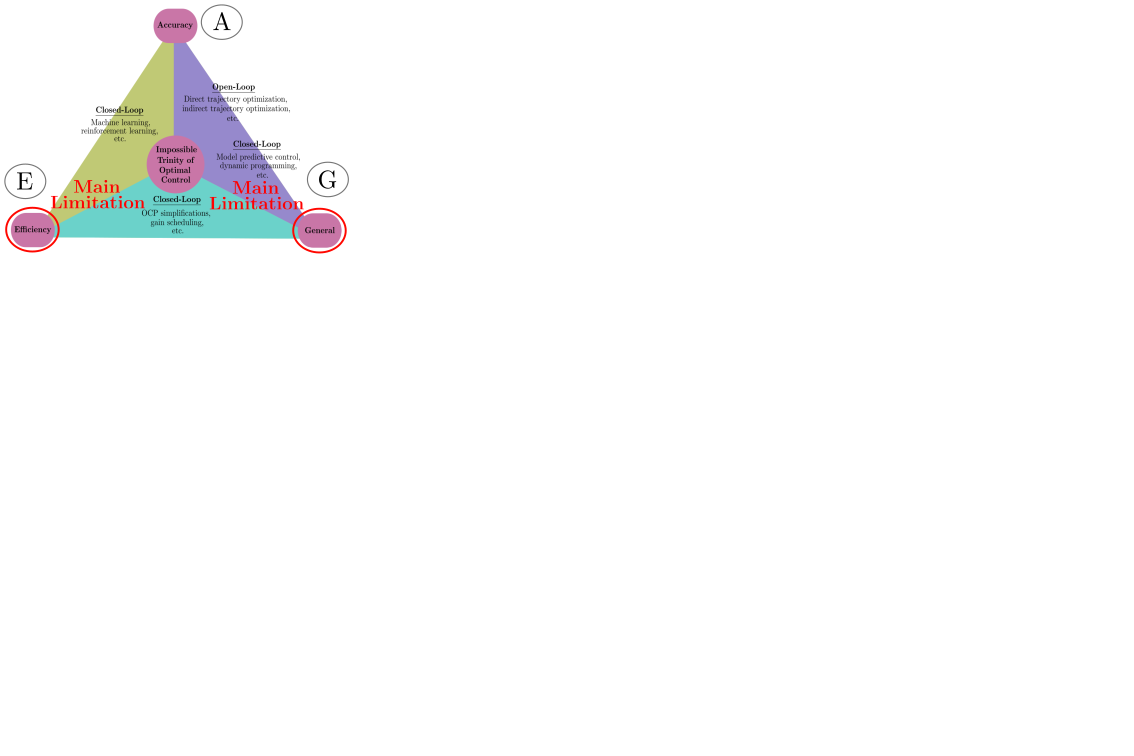
\includegraphics[width=0.84\textwidth]{../figs/sparsehjb/itoc_previous_work_1.png}
                \end{figure}}
            \only<2>{
                \begin{figure}
                    \centering
                    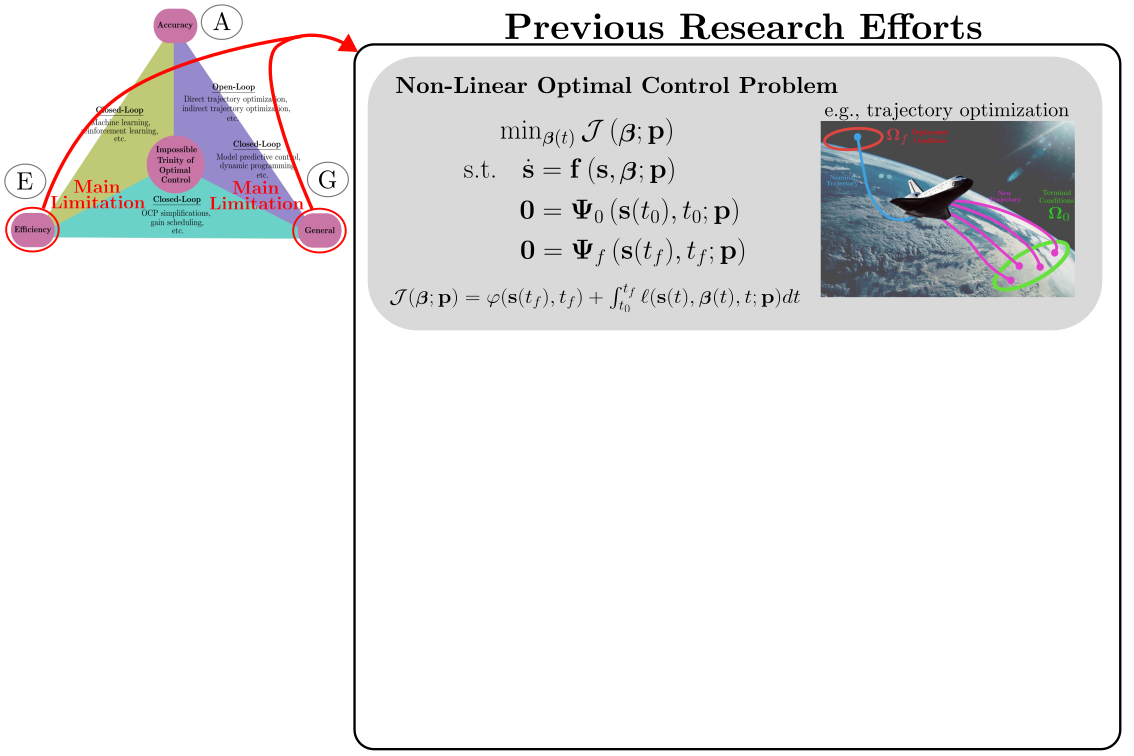
\includegraphics[width=0.84\textwidth]{../figs/sparsehjb/itoc_previous_work_2.png}
                \end{figure}}
            \only<3>{
                \begin{figure}
                    \centering
                    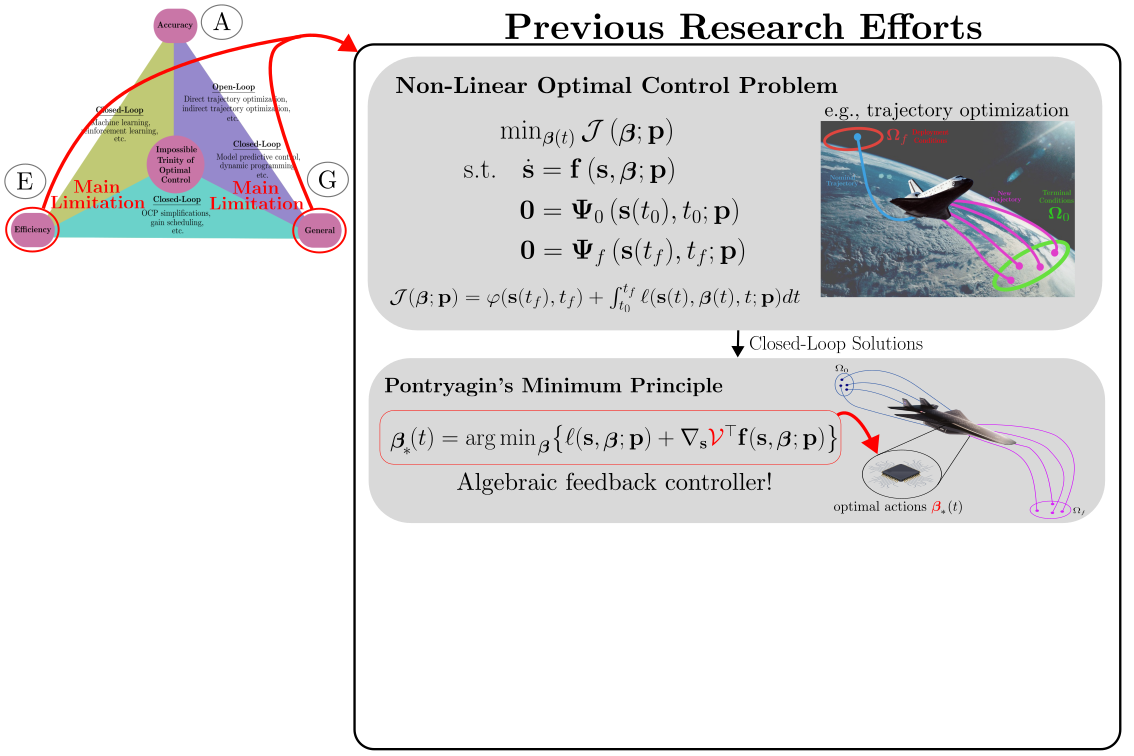
\includegraphics[width=0.84\textwidth]{../figs/sparsehjb/itoc_previous_work_3.png}
                \end{figure}}
            \only<4>{
                \begin{figure}
                    \centering
                    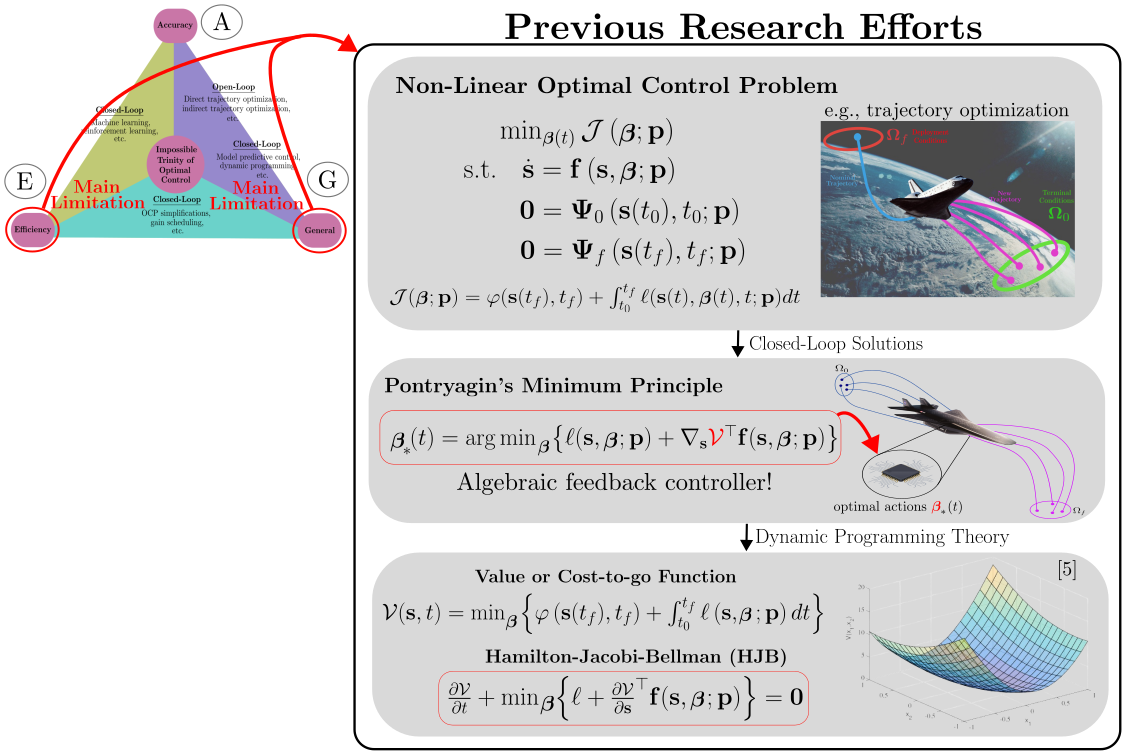
\includegraphics[width=0.84\textwidth]{../figs/sparsehjb/itoc_previous_work_4.png}
                \end{figure}}
            \only<5>{
                \begin{figure}
                    \centering
                    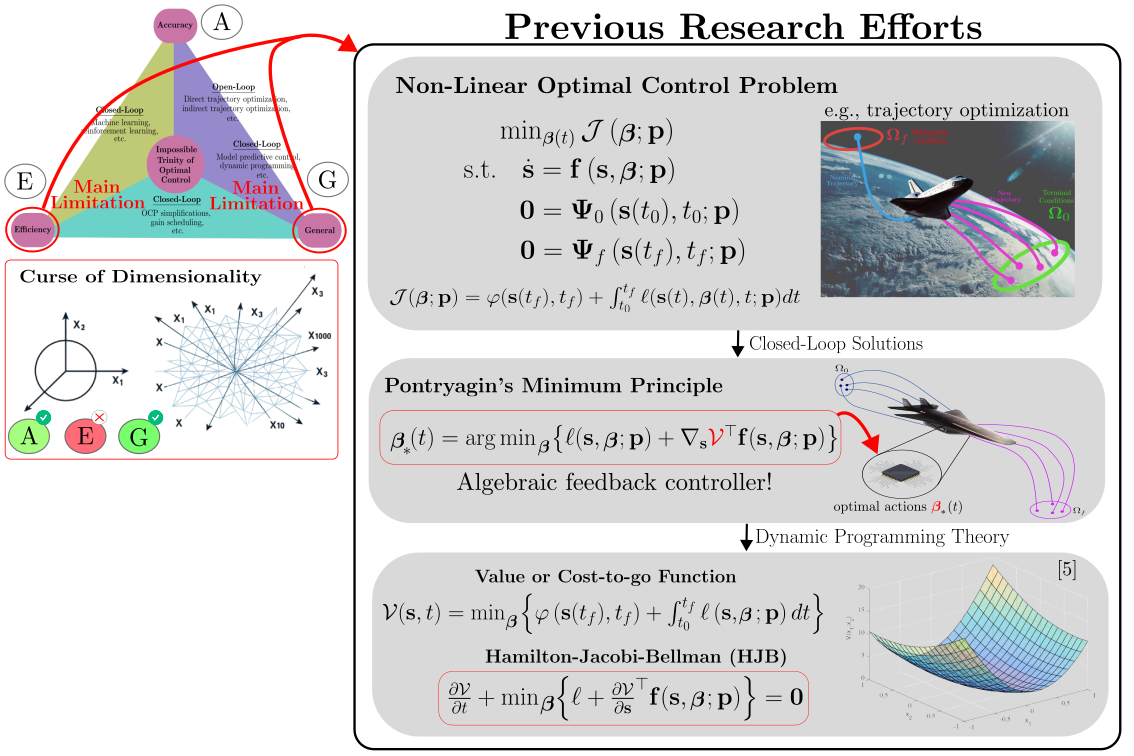
\includegraphics[width=0.84\textwidth]{../figs/sparsehjb/itoc_previous_work_5.png}
                \end{figure}}
            \only<6>{
                \begin{figure}
                    \centering
                    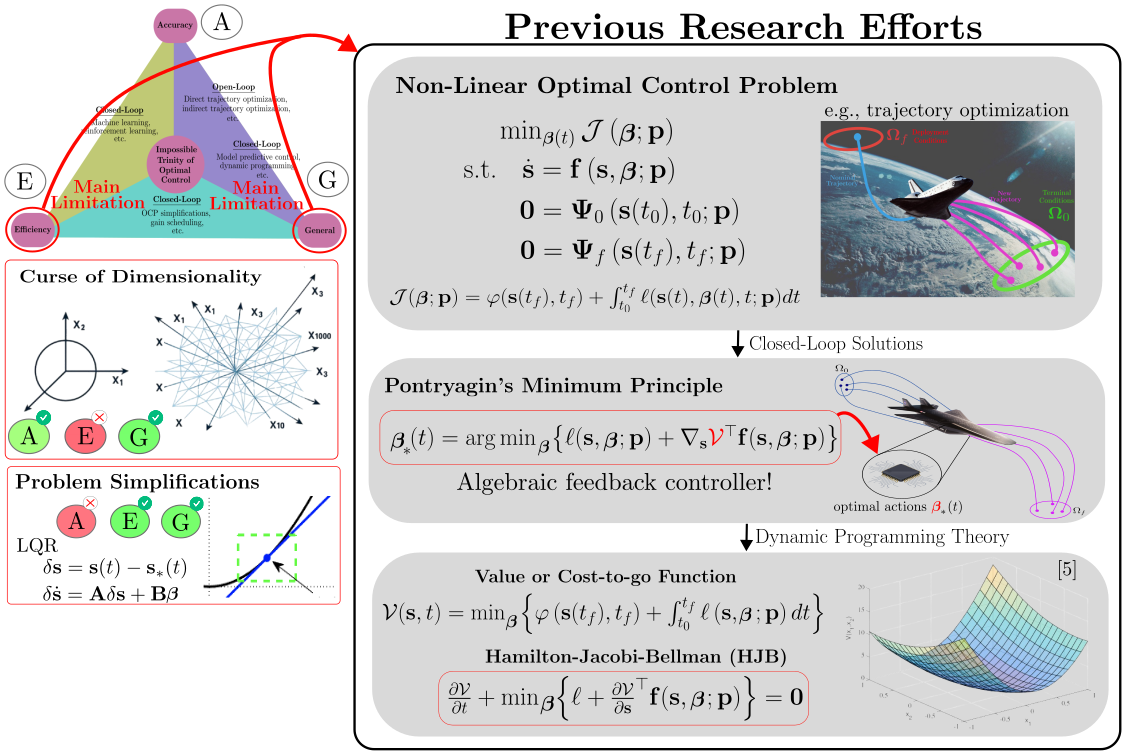
\includegraphics[width=0.84\textwidth]{../figs/sparsehjb/itoc_previous_work_6.png}
                \end{figure}}
            \only<7>{
                \begin{figure}
                    \centering
                    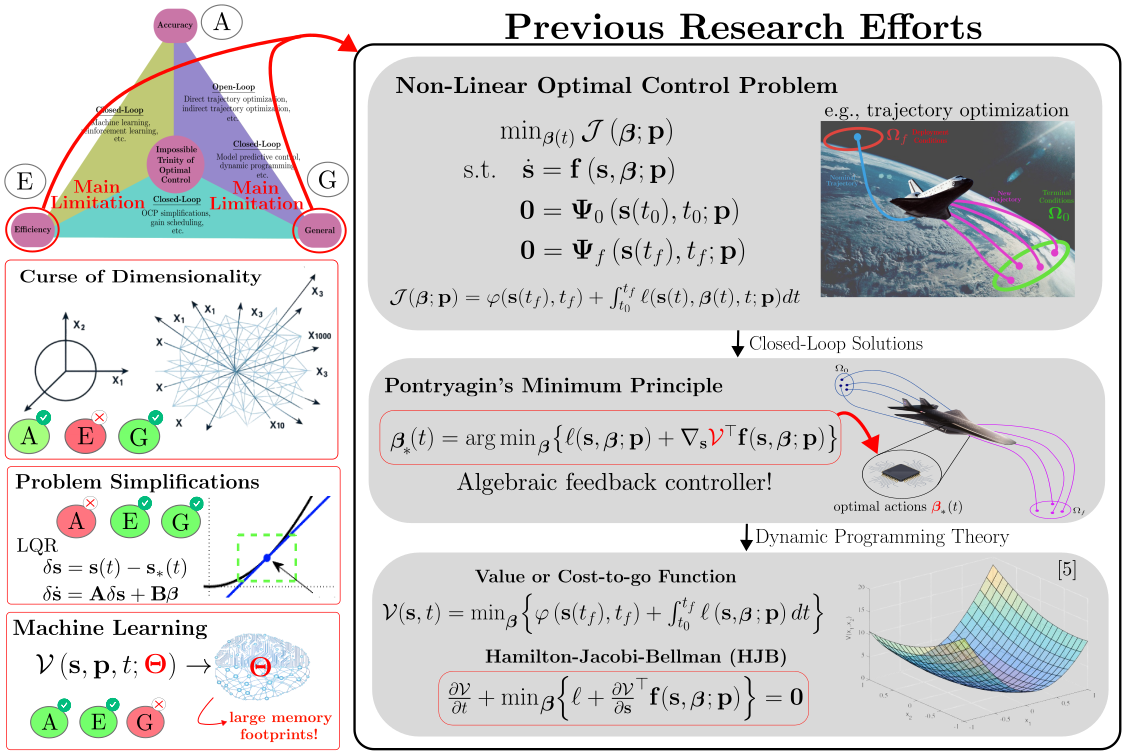
\includegraphics[width=0.84\textwidth]{../figs/sparsehjb/itoc_previous_work_7.png}
                \end{figure}}
        \end{column}
        \hspace*{-0.6in}
        \begin{column}{0.27\textwidth}
            \centering
            \tiny
            \vspace*{-0.1in}
            \visible<2->{
            \begin{graybox}{Optimal Control Problem}
                \begin{itemize}
                    \item $\vs$: system state,
                    \vspace*{-0.05in}
                    \item  $\vp$: OCP parameters,
                    \vspace*{-0.05in}
                    \item $\redvbeta$: control action,
                    \vspace*{-0.05in}
                    \item $\vf$: non-linear dynamics,
                    \vspace*{-0.05in}
                    \item $\vPsi_0$: initial constraints,
                    \vspace*{-0.05in}
                    \item $\vPsi_f$: terminal constraints,
                \end{itemize}
            \end{graybox}}
            \visible<5->{
            \begin{graybox}{We still have problems...}
                \begin{itemize}
                    \item<5-> curse of dimensionality,
                    \vspace*{-0.05in}
                    \item<6-> OCP simplifications,
                    \vspace*{-0.05in}
                    \item<7-> black-box control policies,
                    \vspace*{-0.05in}
                    \item<7-> \colorbox{red!30}{limited data},
                    \vspace*{-0.05in}
                    \item<7-> \colorbox{red!30}{large memory requirements}
                \end{itemize}
            \end{graybox}}
        \end{column}
    \end{columns}
\end{frame}